\documentclass[a4paper]{article}

\usepackage[pdftex]{graphicx}

\setlength{\parindent}{0pt}
\setlength{\parskip}{10pt}
\setlength{\hoffset}{10pt}
\setlength{\marginparsep}{0pt}
\setlength{\oddsidemargin}{0pt}
\setlength{\evensidemargin}{0pt}
\setlength{\textwidth}{410pt}
\setlength{\topmargin}{0pt}
\setlength{\textheight}{645pt}

\newenvironment{twocoltable}{\begin{tabular}{p{3cm}l}}{\end{tabular}}
\def\tilurl{http://til.berlios.de}

\begin{document}
\DeclareGraphicsExtensions{.pdf,.png}

\begin{titlepage}
\vspace*{4cm}
\begin{center}
\huge{Text Input Layer - White Paper}\\
\huge{(Preliminary version)}\\
\vspace{1cm}
\large{Pascal Maillard}\\
\vspace{.5cm}
\large{\today}\\
\vspace{1cm}
\large{\tilurl}\\
\vspace{1cm}
\large{\emph{Important note: This document a preliminary version. The software described in it has \emph{not yet been implemented}, instead, this white paper describes the goals we aim to achieve.}}\\
\end{center}
\vfill
Copyright \copyright\ 2005, Pascal Maillard\\
Permission is granted to copy, distribute and/or modify this document under the terms of the GNU Free Documentation License, Version 1.1 or any later version published by the Free Software Foundation.
\end{titlepage}

\begin{titlepage}
\tableofcontents
\listoffigures
\listoftables
\end{titlepage}

\section{Purpose of this document}

This document describes the basic ideas that led to the development of the Text Input Layer (TIL). It consists of two parts: The first introduces the TIL, describing the motivation behind it, the problems it tries to solve, a comparison with other attempts to solve these problems and the features the TIL offers. The second part deals with its architectural design and how it has been implemented, including other implementations that were thought of.

What this document does \emph{not} contain, is the exact specification of the TIL Application Programmer's Interface (API), there is separate documentation for this task. You can get it at

\tilurl.

\section{Introduction to the Text Input Layer}

\subsection{Motivation}

There are a lot of programs available that are used to edit text documents. These are for example
\begin{itemize}
\item text editors (like \emph{vi} or \emph{emacs})
\item word processors
\item mail programs
\item integrated development environments (IDE).
\end{itemize}

All of these programs edit text documents but with different intentions: Text editors operate on text-only files. Word processors add formatting information, graphics and/or other data to the documents, which adds information that the text alone cannot provide. The main purpose of mail programs and IDEs is not to edit text documents but to send and manage e-mails or aid in the development of computer software, resp. Editing textual information is thus just a necessary task in order to fulfill the main purpose.

Despite the differences in the way these types of programs make use of their textual information, the way the user interacts with the program to edit these texts follows some common \emph{logical concepts} that have become a de-facto standard and are used by nearly all of the programs the author of this document knows of. There is a set of common \emph{actions} the user can perform on the textual information, such as deleting, inserting or moving portions of the text. Nearly all applications provide a way to copy text and paste it at another position. All the major desktop environments even provide a way to transfer text portions between different applications. Most programs allow undoing and redoing changes the user made.

There is also a common way how these actions are specified by the user. Nowadays, applications always provide a cursor, which indicates the position of the text where an action is to be performed. For example, when the user wants to insert a text portion at a specific position in the text, he/she moves the cursor to that position and then presses a mouse button, a key sequence or whatever the application expects. To operate on text entities (i.e. characters) at once, most applications provide a way to select a portion of the text, often with the use of the cursor.

However, in spite of these common \emph{logical} concepts, the \emph{physical} interaction of the user with the computer (i.e. how he interacts with the input devices) can vary considerably between different programs. Most programs work in the following way: Inserting text is done by simply pressing the corresponding keys on the keyboard, text is deleted by pressing the \emph{delete} key and the \emph{insert} key starts a \emph{replace mode}. The cursor is moved with the cursor keys or by clicking with the mouse on a position in the text. Text can be selected either by moving the cursor while pressing \emph{shift} or by dragging the mouse over the text. Text can by copied, cut and pasted with Ctrl-C, Ctrl-X and Ctrl-V, resp.

There are editors however that work differently. The editor \emph{vi}, for example, has several modes. In insert mode, its behavior is similar to the one described above. In command mode, text is deleted by pressing a key sequence starting with 'd', copied by pressing 'y' and replaced by pressing 'c'. The cursor is moved with 'h', 'j', 'k' and 'l' and the visual mode, which is used to select text, is started by pressing 'v'.

You can't tell which behavior is better, it only depends on the user's preferences. The author of this document prefers the \emph{vi}-style over the ``normal'' one because he believes that it allows him to write more efficiently. Others may have different opinions. The problem is that the physical user interface is hard-coded into most editors, may it be a stand-alone editor like \emph{vi}\footnote{That is not entirely true: in vi, you can map commands to arbitrary keys, thus defining your own commands. However, the system of the different modes vi is famous for cannot be changed.} or an embeddable ``widget'' (this is a word that is often used for elements of a graphical user interface) like the text editor widgets that are provided by frameworks such as GTK, Qt or Cocoa. This means that the user has to adopt the editor's user interface even if he/she is used to another one that is based on the same \emph{logical} concepts, so it could be used to fit the same purpose.

This is where the TIL comes in. It can be thought of as a layer between the physical and the logical user input as shown in Figure \ref{fg:input_model}. This way, it provides a way to define several physical user interfaces and transforms the user's input into a common representation of the logical editing actions decribed above. The editor thus can provide more than one way the user can interact with the program. 

\begin{figure}[ht]

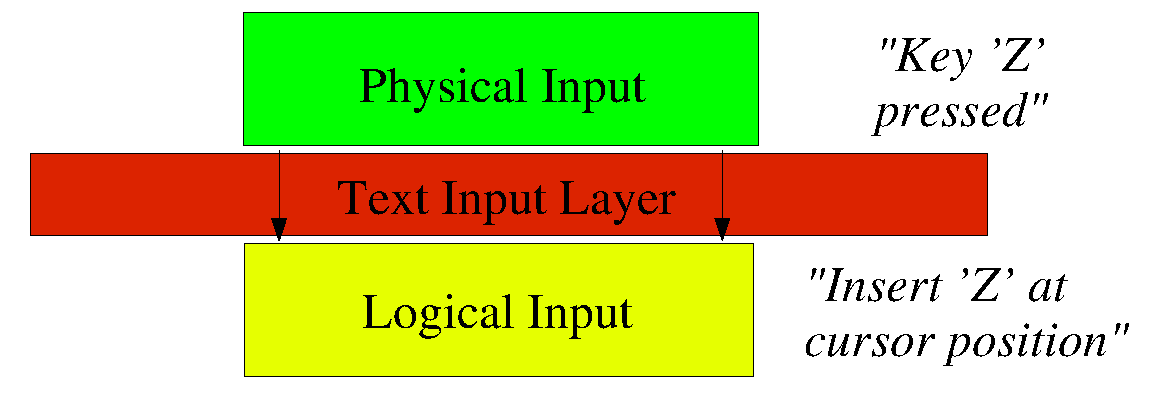
\includegraphics[width=\textwidth]{input_model}

\caption{A model of the user's input}
\label{fg:input_model}
\end{figure}

The author of the TIL has previously helped developing Yzis\footnote{http://www.yzis.org}, a project that tried to solve this issue by creating a \emph{vi}-like editor with a strict separation between logic and user interface (which is not the case with other vi-like editors). Thus, it is easy to create a new user interface and embed it into other applications, which has been done extensively by KDE applications such as KDevelop, Quanta+ or KWrite. However, there are some substantial drawbacks to this approach:

\begin{itemize}
\item A complete text editor has to be reimplemented, including the tasks
  \begin{itemize}
  \item storage of the text, reading/writing it from/to disk
  \item perform the editing actions on the text buffer
  \item undo/redo
  \item advanced features like syntax highlighting, spell checking etc.
  \end{itemize}
\item Yzis probably doesn't integrate well into existing applications, so that it may not provide all the application's features or might look different to the native editor.
\item Yzis only satisfies the (albeit big) \emph{vi} camp, we would like to have a generic way to easily support many input methods.\footnote{The KDE project tried this with the KTextEditor interface, which is also used by Yzis' KDE GUI, but editors written to support this interface still have at least the first two problems, so this is not a perfect solution.}
\end{itemize}

The TIL doesn't have these problems. The only task that has to be implemented is the transformation of the user's input into the logical actions. To be able to use the TIL, a text editor must probably be submitted to some bigger changes, however. Specifically, it must be able to understand the ``language'' in which the TIL describes the logical actions. Additionally, it imposes a separation between physical and logical input on the editor. This need not be a disadvantage, as it leads to a cleaner design. Thus, the TIL cannot only be used to provide an editor with more than one input method, it can also be used to create well-designed editors.

\subsection{Features}

\emph{Important note: As mentioned on the title page, the TIL has not yet been implemented. The ``features'' described here just represent the goals we try to achieve.}

\begin{itemize}
\item support of arbitrary input methods due to the dynamic plugin system
\item ``modern'' and \emph{vi}-like input method available
\item communication between application and TIL is completely done with UTF-8 encoded XML
\item internationalized
\item licensed under the terms of the LGPL and therefore free software
\item written entirely in C (conforming to the ISO/IEC 9899:1999 standard, also known as C99) and runs natively on all major platforms
\item BSD-licensed wrapper code for GTK, Qt and Cocoa available
\end{itemize}

\section{Detailed Description}

\subsection{Architecture}

\begin{figure}[ht]

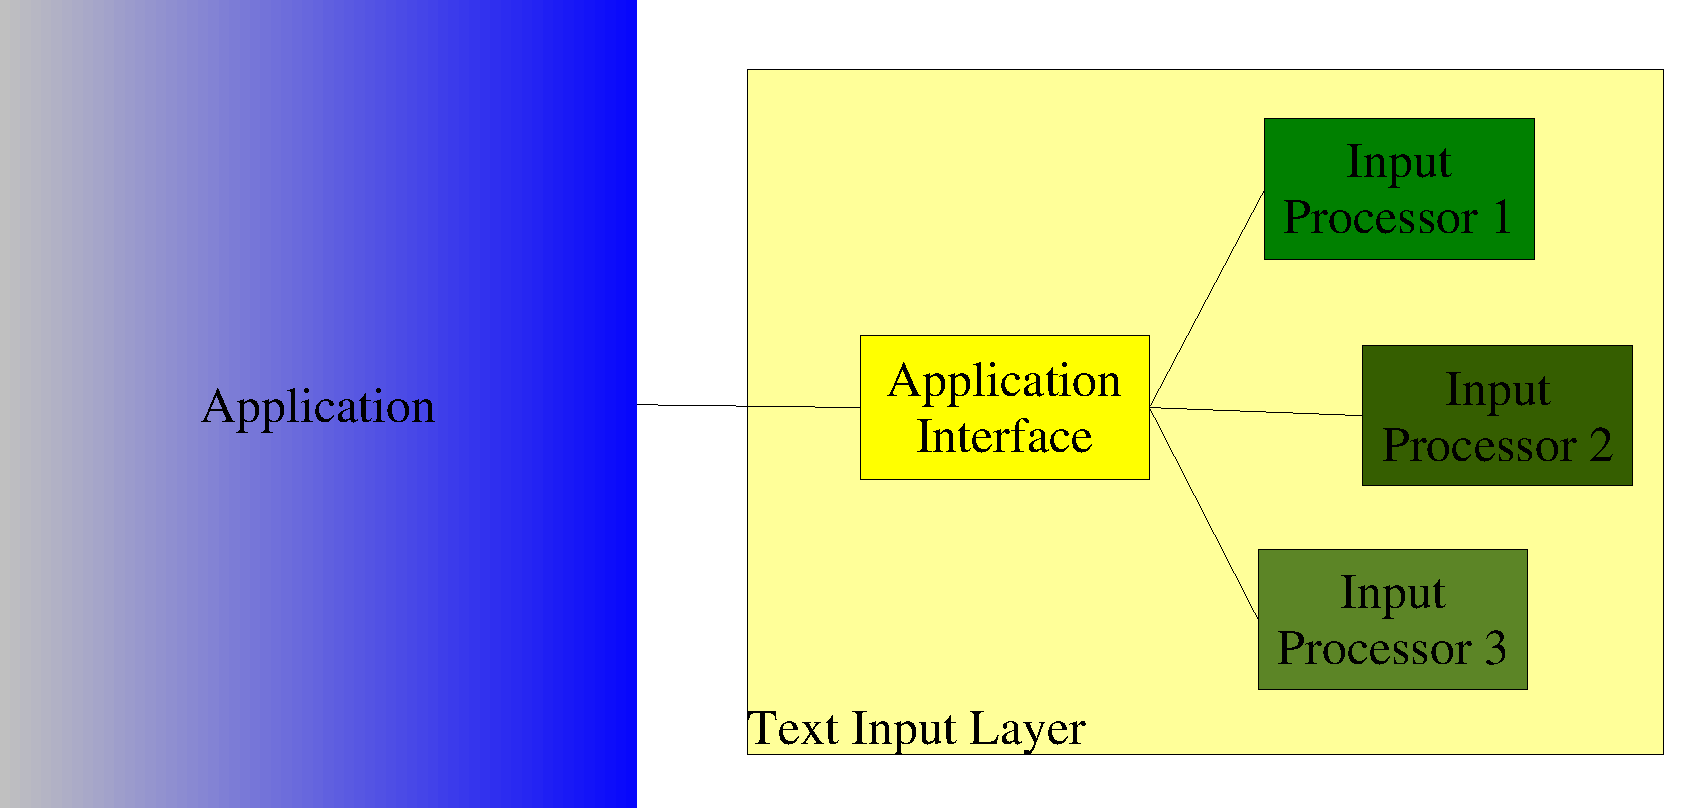
\includegraphics[width=\textwidth]{architecture}

\caption{Architecture}
\label{fg:architecture}
\end{figure}

Figure \ref{fg:architecture} shows the two types of components the TIL is composed of: the \emph{application interface} and the \emph{input processors}. The application interface is the only part the application sees of the TIL. It allows it to load the input processing plugins and change to a specific one at runtime. It further encapsulates the input processors from the application.

These input processor plugins do the real work, which means converting the physical user input into the logical description.

\subsection{Embedding the TIL into an application}

The TIL can easily be embedded into existing applications if there already exists a separation between the physical and the logical input. For example, suppose the application uses Smalltalk's Model-View-Controller (MVC) design as shown in Figure \ref{fg:mvc}. Here, the \emph{text view} is the widget that displays the text and recieves the input events from the window system. These input events are passed on to the \emph{controller}, which ``translates'' them into calls to the \emph{model}.

\begin{figure}[ht]
\centering

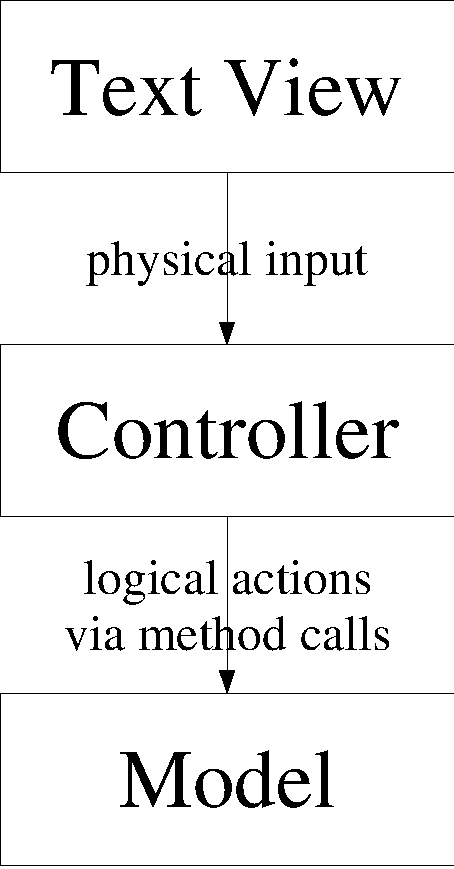
\includegraphics[height=6cm]{mvc}

\caption{Model-View-Controller design}
\label{fg:mvc}
\end{figure}

Thus, the controller does the work the TIL should be doing: translating the physical to the logical input. To integrate the TIL, one only has to change the controller so that it redirects the physical input to the TIL and passes the logical input from the TIL to the model. This is shown in Figure \ref{fg:integration}.

\begin{figure}[ht]
\centering

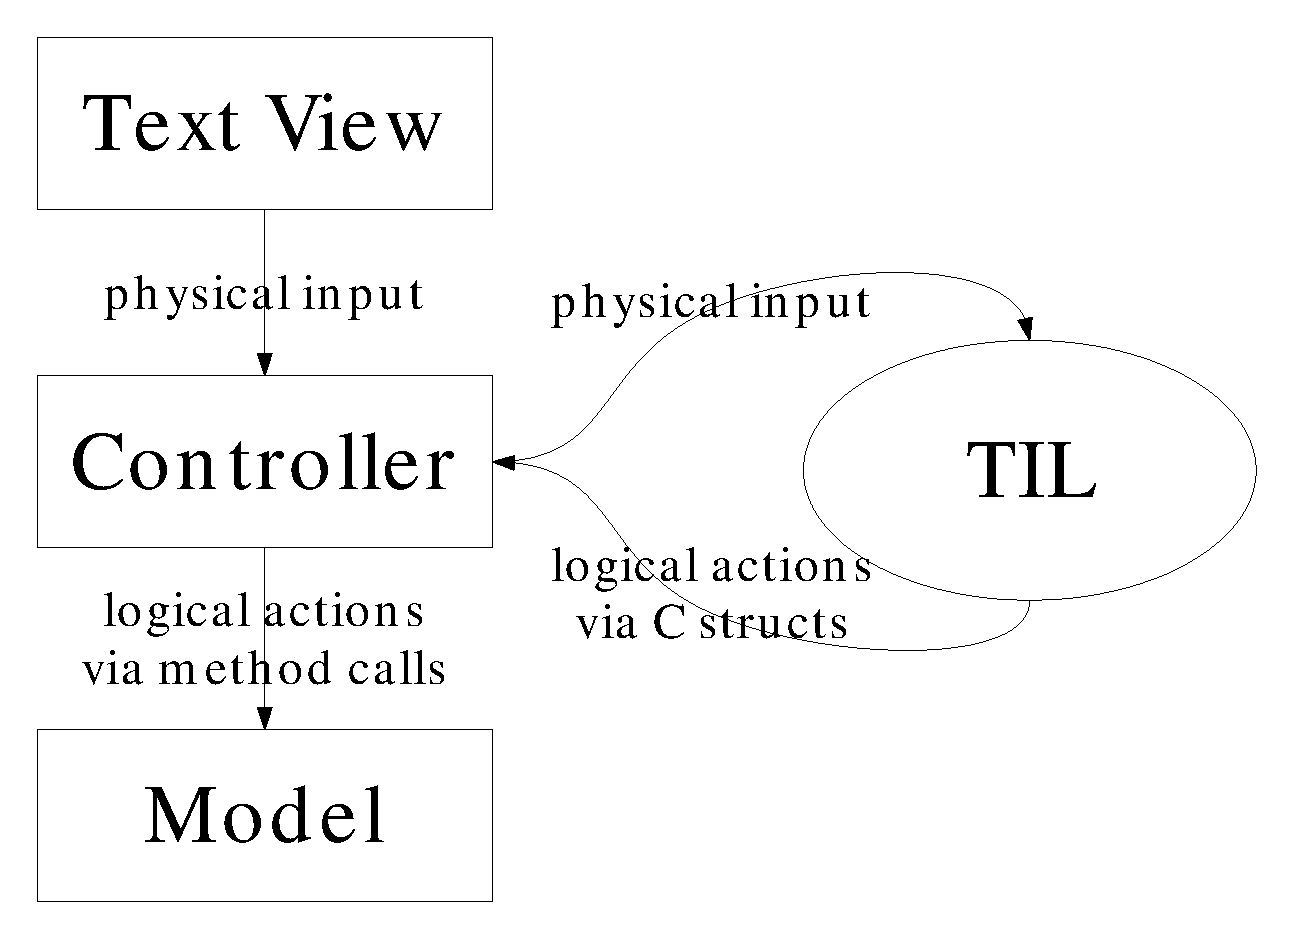
\includegraphics[height=6cm]{integration}

\caption{Integration into an application following the MVC design}
\label{fg:integration}
\end{figure}

\subsection{Implementation}

\begin{figure}[ht]
\centering

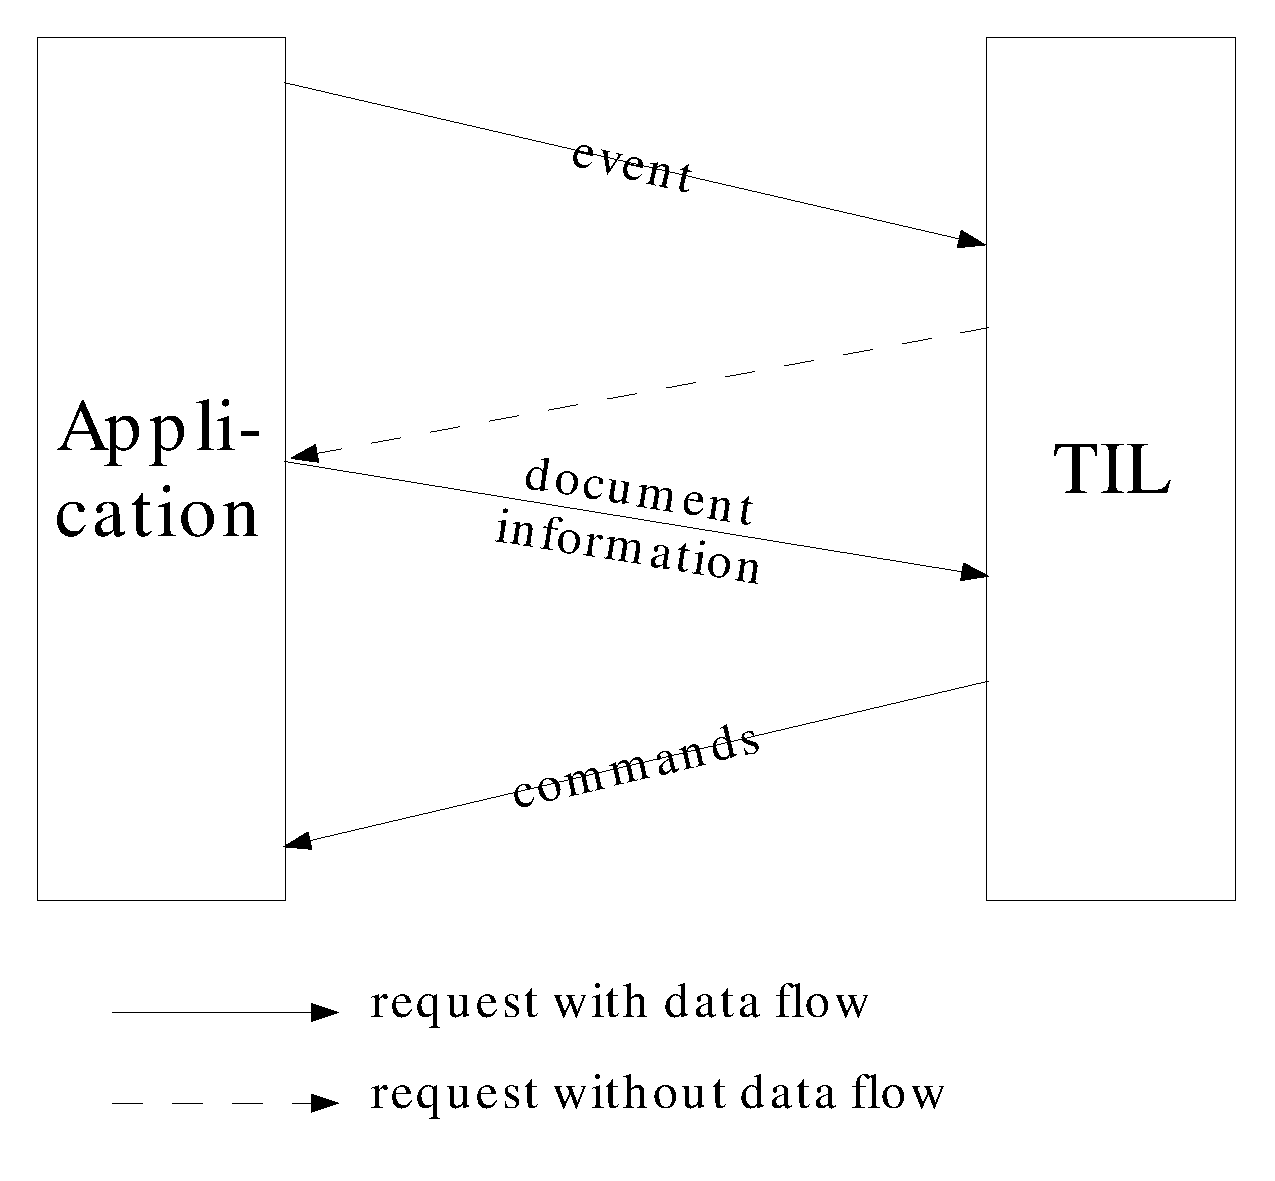
\includegraphics[height=8cm]{dialog}

\caption{A dialog between application and TIL}
\label{fg:dialog}
\end{figure}

The communication between application and TIL can be thought of as a sequence of dialogs. A dialog is always started by the application sending an \emph{event} along with its description to the TIL. This event will most probably be the cause of a user action (e.g. when pressing a key), but can also be triggered otherwise, for example by a timer. The application then waits for the TIL to return with a \emph{command sequence}: a description of what the user told the application to do. Before doing so, the TIL can also query information about the document from the application which can affect its behavior. Figure \ref{fg:dialog} illustrates such a dialog.


A command sequence is an ordered list of zero or more basic commands, which for example tell the application to move the cursor or insert a string in the text. Table \ref{tb:commands} lists the commands currently implemented. They are put in logical groups here for clarity.

\begin{table}[p]
\setlength{\parskip}{10pt}
Cursor and Selection:

\begin{twocoltable}
move:	& move the cursor \\
change cursor:	& set the appearance of the cursor \\
set selection:	& set the selection mode (none, normal, line or block) \\
\end{twocoltable}

Basic Editing: 

\begin{twocoltable}
delete:	& delete a text range \\
insert:	& insert text \\
replace:	& replace text by other text \\
copy:	& copy text to the clipboard \\
\end{twocoltable}

Advanced Editing: 

\begin{twocoltable}
undo:	& undo last operation \\
redo:	& redo last operation \\
indent:	& indent or unindent text \\
complete:	& complete word currently written \\
format:	& format text, e.g. program code, to be more readable \\
\end{twocoltable}

Misc: 

\begin{twocoltable}
open:	& open another document \\
set status text:	& set the status text that is displayed at the bottom \\
\end{twocoltable}
\caption{Available commands}
\label{tb:commands}
\end{table}

Table \ref{tb:categories} shows which groups contain \emph{editing} or \emph{composable} commands.

\emph{Editing} commands are commands that change the document. The application should provide functionality to undo the changes caused by these commands. When doing this, it should treat the changes caused by a whole command sequence atomically, i.e. undoing should revert all the changes caused by this command sequence.

\emph{Composable} commands are commands that can be put together with other commands to form a command sequence as described above. Commands that are not composable must be the only command in such a sequence.

A command sequence also contains a human-readable and internationalized description of what the command sequence is supposed to do. This can be displayed for example when undoing or redoing the changes.

\newpage

\begin{table}[p]
\centering
\begin{tabular}{|l|c|c|}
\hline
\textbf{Command} & \textbf{Editing} & \textbf{Composable}\\
\hline\hline
move	&   & x \\
\hline
change cursor	&   &   \\
\hline
set selection	&   & x \\
\hline
delete	& x & x \\
\hline
insert	& x & x \\
\hline
replace	& x & x \\
\hline
copy	&   & x \\
\hline
undo	& x &   \\
\hline
redo	& x &   \\
\hline
indent	& x & x \\
\hline
complete	& x & x \\
\hline
format	& x & x \\
\hline
open	&   &   \\
\hline
set status text	&   &   \\
\hline
\end{tabular}
\caption{Editing and composable commands}
\label{tb:categories}
\end{table}

\end{document}

% vim: ts=20
